% Options for packages loaded elsewhere
\PassOptionsToPackage{unicode}{hyperref}
\PassOptionsToPackage{hyphens}{url}
%
\documentclass[
]{article}
\usepackage{amsmath,amssymb}
\usepackage{lmodern}
\usepackage{ifxetex,ifluatex}
\ifnum 0\ifxetex 1\fi\ifluatex 1\fi=0 % if pdftex
  \usepackage[T1]{fontenc}
  \usepackage[utf8]{inputenc}
  \usepackage{textcomp} % provide euro and other symbols
\else % if luatex or xetex
  \usepackage{unicode-math}
  \defaultfontfeatures{Scale=MatchLowercase}
  \defaultfontfeatures[\rmfamily]{Ligatures=TeX,Scale=1}
\fi
% Use upquote if available, for straight quotes in verbatim environments
\IfFileExists{upquote.sty}{\usepackage{upquote}}{}
\IfFileExists{microtype.sty}{% use microtype if available
  \usepackage[]{microtype}
  \UseMicrotypeSet[protrusion]{basicmath} % disable protrusion for tt fonts
}{}
\makeatletter
\@ifundefined{KOMAClassName}{% if non-KOMA class
  \IfFileExists{parskip.sty}{%
    \usepackage{parskip}
  }{% else
    \setlength{\parindent}{0pt}
    \setlength{\parskip}{6pt plus 2pt minus 1pt}}
}{% if KOMA class
  \KOMAoptions{parskip=half}}
\makeatother
\usepackage{xcolor}
\IfFileExists{xurl.sty}{\usepackage{xurl}}{} % add URL line breaks if available
\IfFileExists{bookmark.sty}{\usepackage{bookmark}}{\usepackage{hyperref}}
\hypersetup{
  pdftitle={Assignments},
  hidelinks,
  pdfcreator={LaTeX via pandoc}}
\urlstyle{same} % disable monospaced font for URLs
\usepackage[margin=1in]{geometry}
\usepackage{color}
\usepackage{fancyvrb}
\newcommand{\VerbBar}{|}
\newcommand{\VERB}{\Verb[commandchars=\\\{\}]}
\DefineVerbatimEnvironment{Highlighting}{Verbatim}{commandchars=\\\{\}}
% Add ',fontsize=\small' for more characters per line
\usepackage{framed}
\definecolor{shadecolor}{RGB}{248,248,248}
\newenvironment{Shaded}{\begin{snugshade}}{\end{snugshade}}
\newcommand{\AlertTok}[1]{\textcolor[rgb]{0.94,0.16,0.16}{#1}}
\newcommand{\AnnotationTok}[1]{\textcolor[rgb]{0.56,0.35,0.01}{\textbf{\textit{#1}}}}
\newcommand{\AttributeTok}[1]{\textcolor[rgb]{0.77,0.63,0.00}{#1}}
\newcommand{\BaseNTok}[1]{\textcolor[rgb]{0.00,0.00,0.81}{#1}}
\newcommand{\BuiltInTok}[1]{#1}
\newcommand{\CharTok}[1]{\textcolor[rgb]{0.31,0.60,0.02}{#1}}
\newcommand{\CommentTok}[1]{\textcolor[rgb]{0.56,0.35,0.01}{\textit{#1}}}
\newcommand{\CommentVarTok}[1]{\textcolor[rgb]{0.56,0.35,0.01}{\textbf{\textit{#1}}}}
\newcommand{\ConstantTok}[1]{\textcolor[rgb]{0.00,0.00,0.00}{#1}}
\newcommand{\ControlFlowTok}[1]{\textcolor[rgb]{0.13,0.29,0.53}{\textbf{#1}}}
\newcommand{\DataTypeTok}[1]{\textcolor[rgb]{0.13,0.29,0.53}{#1}}
\newcommand{\DecValTok}[1]{\textcolor[rgb]{0.00,0.00,0.81}{#1}}
\newcommand{\DocumentationTok}[1]{\textcolor[rgb]{0.56,0.35,0.01}{\textbf{\textit{#1}}}}
\newcommand{\ErrorTok}[1]{\textcolor[rgb]{0.64,0.00,0.00}{\textbf{#1}}}
\newcommand{\ExtensionTok}[1]{#1}
\newcommand{\FloatTok}[1]{\textcolor[rgb]{0.00,0.00,0.81}{#1}}
\newcommand{\FunctionTok}[1]{\textcolor[rgb]{0.00,0.00,0.00}{#1}}
\newcommand{\ImportTok}[1]{#1}
\newcommand{\InformationTok}[1]{\textcolor[rgb]{0.56,0.35,0.01}{\textbf{\textit{#1}}}}
\newcommand{\KeywordTok}[1]{\textcolor[rgb]{0.13,0.29,0.53}{\textbf{#1}}}
\newcommand{\NormalTok}[1]{#1}
\newcommand{\OperatorTok}[1]{\textcolor[rgb]{0.81,0.36,0.00}{\textbf{#1}}}
\newcommand{\OtherTok}[1]{\textcolor[rgb]{0.56,0.35,0.01}{#1}}
\newcommand{\PreprocessorTok}[1]{\textcolor[rgb]{0.56,0.35,0.01}{\textit{#1}}}
\newcommand{\RegionMarkerTok}[1]{#1}
\newcommand{\SpecialCharTok}[1]{\textcolor[rgb]{0.00,0.00,0.00}{#1}}
\newcommand{\SpecialStringTok}[1]{\textcolor[rgb]{0.31,0.60,0.02}{#1}}
\newcommand{\StringTok}[1]{\textcolor[rgb]{0.31,0.60,0.02}{#1}}
\newcommand{\VariableTok}[1]{\textcolor[rgb]{0.00,0.00,0.00}{#1}}
\newcommand{\VerbatimStringTok}[1]{\textcolor[rgb]{0.31,0.60,0.02}{#1}}
\newcommand{\WarningTok}[1]{\textcolor[rgb]{0.56,0.35,0.01}{\textbf{\textit{#1}}}}
\usepackage{graphicx}
\makeatletter
\def\maxwidth{\ifdim\Gin@nat@width>\linewidth\linewidth\else\Gin@nat@width\fi}
\def\maxheight{\ifdim\Gin@nat@height>\textheight\textheight\else\Gin@nat@height\fi}
\makeatother
% Scale images if necessary, so that they will not overflow the page
% margins by default, and it is still possible to overwrite the defaults
% using explicit options in \includegraphics[width, height, ...]{}
\setkeys{Gin}{width=\maxwidth,height=\maxheight,keepaspectratio}
% Set default figure placement to htbp
\makeatletter
\def\fps@figure{htbp}
\makeatother
\setlength{\emergencystretch}{3em} % prevent overfull lines
\providecommand{\tightlist}{%
  \setlength{\itemsep}{0pt}\setlength{\parskip}{0pt}}
\setcounter{secnumdepth}{-\maxdimen} % remove section numbering
\ifluatex
  \usepackage{selnolig}  % disable illegal ligatures
\fi

\title{Assignments}
\author{}
\date{\vspace{-2.5em}}

\begin{document}
\maketitle

{
\setcounter{tocdepth}{1}
\tableofcontents
}
This page contains all of my assignments for the class.

\hypertarget{assignment-1}{%
\section{Assignment 1}\label{assignment-1}}

\textbf{Collaborators: Tori Borlase and Halle Wasser. }

\hypertarget{problem-1}{%
\subsubsection{Problem 1}\label{problem-1}}

Install the datasets package on the console below using
\texttt{install.packages("datasets")}. Now load the library.

\begin{Shaded}
\begin{Highlighting}[]
\CommentTok{\#install.packages("datasets")}
\FunctionTok{library}\NormalTok{(datasets)}
\end{Highlighting}
\end{Shaded}

\textbf{Now, it's installed!}

Load the USArrests dataset and rename it \texttt{dat}. Note that this
dataset comes with R, in the package datasets, so there's no need to
load data from your computer. Why is it useful to rename the dataset?

\begin{Shaded}
\begin{Highlighting}[]
\NormalTok{dat}\OtherTok{\textless{}{-}}\NormalTok{USArrests}
\end{Highlighting}
\end{Shaded}

\textbf{Answer: It is useful to rename the dataset because it allows for
replication. Renaming the dataset serves essentially the same function
as ``Save as'' on a word document, which allows you to save the current
version separately and still have access to previous versions. In other
words, renaming the dataset allows you to perform functions without
contaminating the original data.}

\hypertarget{problem-2}{%
\subsubsection{Problem 2}\label{problem-2}}

Use this command to make the state names into a new variable called
State.

\begin{Shaded}
\begin{Highlighting}[]
\NormalTok{dat}\SpecialCharTok{$}\NormalTok{state}\OtherTok{\textless{}{-}}\FunctionTok{tolower}\NormalTok{(}\FunctionTok{rownames}\NormalTok{(USArrests))}
\end{Highlighting}
\end{Shaded}

This dataset has the state names as row names, so we just want to make
them into a new variable. We also make them all lower case, because that
will help us draw a map later - the map function requires the states to
be lower case.

List the variables contained in the dataset \texttt{USArrests}.

\begin{Shaded}
\begin{Highlighting}[]
\FunctionTok{names}\NormalTok{(dat)}
\end{Highlighting}
\end{Shaded}

\begin{verbatim}
## [1] "Murder"   "Assault"  "UrbanPop" "Rape"
\end{verbatim}

\textbf{Answer: The variables contained in the dataset are Murder,
Assualt, UrbanPop (Urban Population), Rape, and state. }

\hypertarget{problem-3}{%
\subsubsection{Problem 3}\label{problem-3}}

What type of variable (from the DVB chapter) is \texttt{Murder}?

\textbf{Answer: According to the DVB chapter, Murder is a quantitative
variable because it measures how many murder arrests were made per
100,000 people}

What R Type of variable is it?

\begin{Shaded}
\begin{Highlighting}[]
\FunctionTok{typeof}\NormalTok{(}\StringTok{"Murder"}\NormalTok{)}
\end{Highlighting}
\end{Shaded}

\begin{verbatim}
## [1] "character"
\end{verbatim}

\textbf{Answer: The typeof() function just tells us what type of object
is within the parenthesis. Therefore, although the R output states that
``Murder'' is a character, it is actually a numeric variable}

\hypertarget{problem-4}{%
\subsubsection{Problem 4}\label{problem-4}}

What information is contained in this dataset, in general? What do the
numbers mean?

\begin{Shaded}
\begin{Highlighting}[]
\FunctionTok{head}\NormalTok{(dat)}
\end{Highlighting}
\end{Shaded}

\begin{verbatim}
##            Murder Assault UrbanPop Rape
## Alabama      13.2     236       58 21.2
## Alaska       10.0     263       48 44.5
## Arizona       8.1     294       80 31.0
## Arkansas      8.8     190       50 19.5
## California    9.0     276       91 40.6
## Colorado      7.9     204       78 38.7
\end{verbatim}

\textbf{Answer: In general, information about how many arrests were made
for murder, assault, and rape per 100,000 people in each state is
contained in this dataset. This dataset also contains the percent urban
population for each state.}

\hypertarget{problem-5}{%
\subsubsection{Problem 5}\label{problem-5}}

Draw a histogram of \texttt{Murder} with proper labels and title.

\begin{Shaded}
\begin{Highlighting}[]
\FunctionTok{hist}\NormalTok{(dat}\SpecialCharTok{$}\NormalTok{Murder, }\AttributeTok{main=}\StringTok{"Frequency of Murder Arrest Rates in the United States"}\NormalTok{, }\AttributeTok{xlab =} \StringTok{"Murder Arrests per 100,000"}\NormalTok{, }\AttributeTok{border=}\StringTok{"black"}\NormalTok{, }\AttributeTok{col =} \StringTok{"blue"}\NormalTok{, }\AttributeTok{xlim=} \FunctionTok{c}\NormalTok{(}\DecValTok{0}\NormalTok{,}\DecValTok{20}\NormalTok{))}
\end{Highlighting}
\end{Shaded}

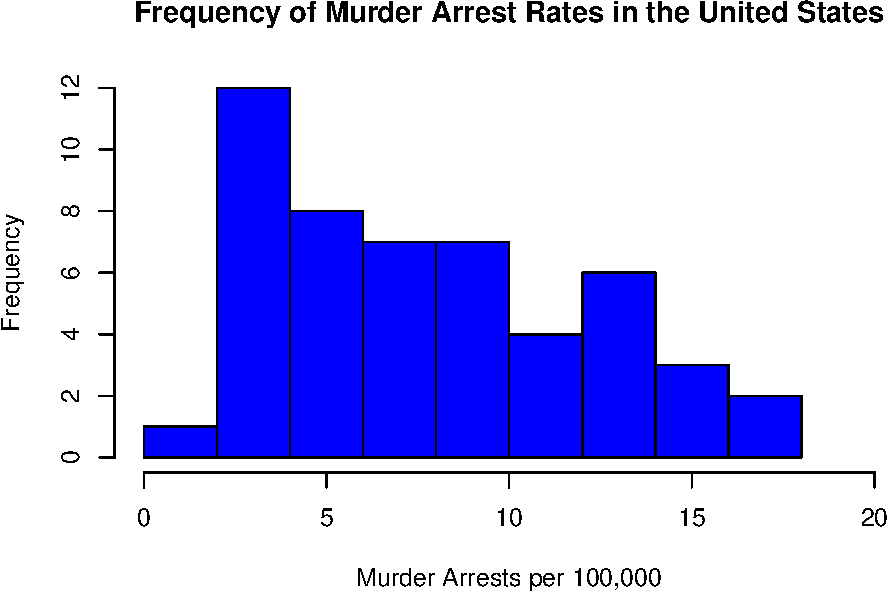
\includegraphics{Assignments_files/figure-latex/unnamed-chunk-7-1.pdf}

\hypertarget{problem-6}{%
\subsubsection{Problem 6}\label{problem-6}}

Please summarize \texttt{Murder} quantitatively. What are its mean and
median? What is the difference between mean and median? What is a
quartile, and why do you think R gives you the 1st Qu. and 3rd Qu.?

\begin{Shaded}
\begin{Highlighting}[]
\FunctionTok{mean}\NormalTok{(dat}\SpecialCharTok{$}\NormalTok{Murder)}
\end{Highlighting}
\end{Shaded}

\begin{verbatim}
## [1] 7.788
\end{verbatim}

\begin{Shaded}
\begin{Highlighting}[]
\FunctionTok{median}\NormalTok{(dat}\SpecialCharTok{$}\NormalTok{Murder)}
\end{Highlighting}
\end{Shaded}

\begin{verbatim}
## [1] 7.25
\end{verbatim}

\begin{Shaded}
\begin{Highlighting}[]
\FunctionTok{quantile}\NormalTok{(dat}\SpecialCharTok{$}\NormalTok{Murder)}
\end{Highlighting}
\end{Shaded}

\begin{verbatim}
##     0%    25%    50%    75%   100% 
##  0.800  4.075  7.250 11.250 17.400
\end{verbatim}

\textbf{Answer: The mean and median of ``Murder'' are 7.788 and 7.25,
respectively. The mean is the average of all the data points (i.e.~the
sum of all the data values divided by the number of values). The median
is the middle value when the data is arranged in order and it provides
information regarding robustness. A quartile is a type of quantile that
divides the data set into 4 (roughly) equally-sized parts
(i.e.~quarters) when the data is arranged from smallest to largest
value. Therefore, quartiles serve to measure the spread of values above
and below the mean. R gives us the 1st and 3rd quartiles because the 2nd
quartile is the same as the median. As you can see in the output above,
the value associated with 50\% is the same as the median (because 50\%
of the values in the data set are above this value). }

\hypertarget{problem-7}{%
\subsubsection{Problem 7}\label{problem-7}}

Repeat the same steps you followed for \texttt{Murder}, for the
variables \texttt{Assault} and \texttt{Rape}. Now plot all three
histograms together. You can do this by using the command
\texttt{par(mfrow=c(3,1))} and then plotting each of the three.

\begin{Shaded}
\begin{Highlighting}[]
\CommentTok{\#Assault}
\FunctionTok{mean}\NormalTok{(dat}\SpecialCharTok{$}\NormalTok{Assault)}
\end{Highlighting}
\end{Shaded}

\begin{verbatim}
## [1] 170.76
\end{verbatim}

\begin{Shaded}
\begin{Highlighting}[]
\FunctionTok{median}\NormalTok{(dat}\SpecialCharTok{$}\NormalTok{Assault)}
\end{Highlighting}
\end{Shaded}

\begin{verbatim}
## [1] 159
\end{verbatim}

\begin{Shaded}
\begin{Highlighting}[]
\FunctionTok{quantile}\NormalTok{(dat}\SpecialCharTok{$}\NormalTok{Assault)}
\end{Highlighting}
\end{Shaded}

\begin{verbatim}
##   0%  25%  50%  75% 100% 
##   45  109  159  249  337
\end{verbatim}

\begin{Shaded}
\begin{Highlighting}[]
\CommentTok{\#Rape}
\FunctionTok{mean}\NormalTok{(dat}\SpecialCharTok{$}\NormalTok{Rape)}
\end{Highlighting}
\end{Shaded}

\begin{verbatim}
## [1] 21.232
\end{verbatim}

\begin{Shaded}
\begin{Highlighting}[]
\FunctionTok{median}\NormalTok{(dat}\SpecialCharTok{$}\NormalTok{Rape)}
\end{Highlighting}
\end{Shaded}

\begin{verbatim}
## [1] 20.1
\end{verbatim}

\begin{Shaded}
\begin{Highlighting}[]
\FunctionTok{quantile}\NormalTok{(dat}\SpecialCharTok{$}\NormalTok{Rape)}
\end{Highlighting}
\end{Shaded}

\begin{verbatim}
##     0%    25%    50%    75%   100% 
##  7.300 15.075 20.100 26.175 46.000
\end{verbatim}

\begin{Shaded}
\begin{Highlighting}[]
\FunctionTok{par}\NormalTok{(}\AttributeTok{mfrow=}\FunctionTok{c}\NormalTok{(}\DecValTok{3}\NormalTok{,}\DecValTok{1}\NormalTok{))}
\FunctionTok{hist}\NormalTok{(dat}\SpecialCharTok{$}\NormalTok{Murder, }\AttributeTok{main=}\StringTok{"Frequency of Murder Arrest Rates in the United States"}\NormalTok{, }\AttributeTok{xlab =} \StringTok{"Murder Arrests per 100,000"}\NormalTok{, }\AttributeTok{border=}\StringTok{"black"}\NormalTok{, }\AttributeTok{col =} \StringTok{"Purple"}\NormalTok{)}
\FunctionTok{hist}\NormalTok{(dat}\SpecialCharTok{$}\NormalTok{Assault, }\AttributeTok{main=}\StringTok{"Frequency of Assault Arrest Rates in the United States"}\NormalTok{, }\AttributeTok{xlab =} \StringTok{"Assault Arrests per 100,000"}\NormalTok{, }\AttributeTok{border=}\StringTok{"black"}\NormalTok{, }\AttributeTok{col =} \StringTok{"Red"}\NormalTok{)}
\FunctionTok{hist}\NormalTok{(dat}\SpecialCharTok{$}\NormalTok{Rape, }\AttributeTok{main=}\StringTok{"Frequency of Rape Arrest Rates in the United States"}\NormalTok{, }\AttributeTok{xlab =} \StringTok{"Rape Arrests per 100,000"}\NormalTok{, }\AttributeTok{border=}\StringTok{"black"}\NormalTok{, }\AttributeTok{col =} \StringTok{"Green"}\NormalTok{)}
\end{Highlighting}
\end{Shaded}

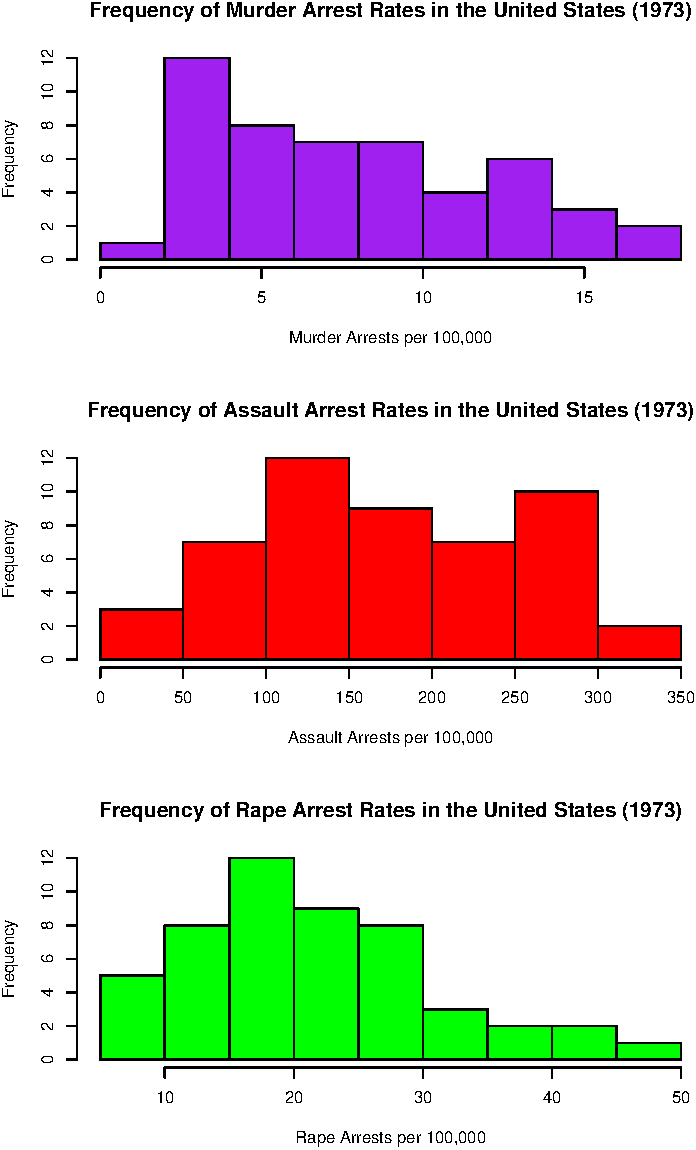
\includegraphics{Assignments_files/figure-latex/unnamed-chunk-11-1.pdf}

What does the command par do, in your own words (you can look this up by
asking R \texttt{?par})?

\textbf{Answer: The R command `par' can be used to combine plots into
one cohesive graph. }

What can you learn from plotting the histograms together?

\textbf{Answer: By plotting the histograms together, we can learn that
histograms for Rape and Murder are (relatively) right-skewed whereas the
histogram for Assault is closer to a normal distribution. }

\hypertarget{problem-8}{%
\subsubsection{Problem 8}\label{problem-8}}

In the console below (not in text), type
\texttt{install.packages("maps")} and press Enter, and then type
\texttt{install.packages("ggplot2")} and press Enter. This will install
the packages so you can load the libraries.

Run this code:

\begin{Shaded}
\begin{Highlighting}[]
\CommentTok{\#install.packages("maps") }
\CommentTok{\#this installs the maps package, which allows the program to draw geographical maps.}
\CommentTok{\#install.packages("ggplot2") }
\CommentTok{\#this installs the ggplot2 program, which allows the program to create elegant data visualizations using the Grammar of Graphics. In other words, it allows for very complex plots/graphics to be created within a data frame. }
\FunctionTok{library}\NormalTok{(}\StringTok{\textquotesingle{}maps\textquotesingle{}}\NormalTok{)  }
\CommentTok{\#this line loads the newly{-}installed "maps" packages}
\FunctionTok{library}\NormalTok{(}\StringTok{\textquotesingle{}ggplot2\textquotesingle{}}\NormalTok{) }
\CommentTok{\#this line loads the newly{-}installed "ggplot2" package}

\FunctionTok{ggplot}\NormalTok{(dat, }\FunctionTok{aes}\NormalTok{(}\AttributeTok{map\_id=}\NormalTok{state, }\AttributeTok{fill=}\NormalTok{Murder)) }\SpecialCharTok{+} 
  \FunctionTok{geom\_map}\NormalTok{(}\AttributeTok{map=}\FunctionTok{map\_data}\NormalTok{(}\StringTok{"state"}\NormalTok{)) }\SpecialCharTok{+} 
  \FunctionTok{expand\_limits}\NormalTok{(}\AttributeTok{x=}\FunctionTok{map\_data}\NormalTok{(}\StringTok{"state"}\NormalTok{)}\SpecialCharTok{$}\NormalTok{long, }\AttributeTok{y=}\FunctionTok{map\_data}\NormalTok{(}\StringTok{"state"}\NormalTok{)}\SpecialCharTok{$}\NormalTok{lat)}
\CommentTok{\#this long line of code reflects the 3 fundamental parts of the ggplot: data, aesthetics, and geometry. It tells the program to use the Murder data from dat and the new "state" variable that we create in Problem 2. It also indicates the x and y variables such that they are instead reflecting latitude and longitude. }
\end{Highlighting}
\end{Shaded}

What does this code do? Explain what each line is doing.

\emph{Answer is commented out above}

\[\\[2in]\]

\hypertarget{assignment-2}{%
\section{Assignment 2}\label{assignment-2}}

(Coming soon)

\end{document}
